\chapter{INTERAÇÃO E PARTICIPAÇÃO}

Das obras destinadas apenas à visualização, passando por inúmeros processos participativos e chegando, finalmente, às questões de interatividade, percebemos mudanças circunstanciais e definitivas em todo o processo artístico ao longo da História da Arte – processo esse, que compreende o momento do insight – a criação, produção e também a recepção e percepção da obra por parte do público. \cite{vares} 

Contudo, é também importante apreender o modo como se estruturam e se organizam
as diferentes possibilidades de interação, com base na premissa de que o procedimento
poético-tecnológico é determinante na produção e, por conseguinte, na recepção de uma
imagem interativa. Neste sentido, nossa intenção será agora estabelecer diferentes níveis de interatividade tomados em função do modo de apropriação da obra pelo receptor. \cite{tavares}

O fenômeno da interação mediado pelas tecnologias eletrônicas pressupõe-se como
um processo de realimentação, em que cada ação do receptor condiciona uma conseqüente
re-ação da máquina (e vice-versa), possibilitando um contínuo diálogo entre esses elementos. \cite{tavares}


Na participação o sujeito submete-se a um sistema pré-estabelecido para poder participar
do mesmo. Já na interatividade o indivíduo interage de forma pontual de
acordo com necessidades pontuais demandadas pela obra.\cite[p. 1140]{semeler2015}


\section{DA CONTEMPLAÇÃO À INTERAÇÃO}

De acordo com \citeonline[p. 97]{frechiani}, historicamente, dentre as tendências que situam a importância do espectador na costituição da obra, a arte percorreu um caminho até finalmente desembocar no universo da interatividade. Esse percurso parte da contemplação, onde o fruidor é um agente passivo, passa pela participação ativa, onde encontramos a manipulação de objetos, até finalmente chegar na interação, onde se manifesta uma relação de reciprocidade entre o usuário e um sistema computacional. 

Segundo \citeonline{plaza}, foi a partir dos anos cinqüenta que se constituiram, no campo da arte, tendências que traduzem e antecipam as mudanças produzidas pelas tecnologias. O artista se interessa por uma nova forma de comunicação, onde procura a participação do espectador para elaborar a obra de arte, modificando assim o estatuto desta e do autor. A obra deixa de ser fruto apenas do artista e se produz no decorrer do diálogo. O espectador não está mais reduzido ao olhar, ele tem a possibilidade de agir sobre a obra e modificá-la, tornando-se co-autor. Ainda de acordo com \citeonline[p. 14]{plaza} "a noção de arte de participação tem por objetivo encurtar a distância entre criador e espectador. Na participação ativa o espectador se vê induzido à manipulação e exploração do objeto artístico ou de seu espaço". Vivenciamos o início do deslocamento das atribuições do artista para o fruidor. 

\citeonline[p. 22]{domingues} afirma que "a obra interativa pede a participação, a colaboração e só tem existência quando é ativada e modificada em tempo real dando respostas instantâneas para quem as experimenta". A visão computacional tem um grande papel nessa dinâmica pois são os algoritmos que tornam os trabalhos artísticos mais interativos, imersivos e fazem com que o espectador se constitua como parte da obra. Como visão computacional compreende-se a definição proposta por \citeonline[p. 134]{caetano} que diz "é a forma pela qual 'o computador enxerga' e 'interpreta as imagens', um conjunto de dados numéricos digitais, uma matriz numérica digital descrevendo qualquer conjunto imagético fisicamente contextualizado".

A arte interativa é, portanto, completamente avessa ao principio da inércia. \citeonline[p. 22]{domingues} conclui que surge um novo espectador mais participativo e que, através das interfaces, tem acesso a obra proposta. São as interfaces amigáveis que permitem as trocas do espectador com as fontes de informação. A contemplação é substituída pela relação. Assim, de acordo com \citeonline[p. 20]{plaza} uma obra de arte interativa é um espaço latente e suscetível a todos os prolongamentos sonoros, visuais e textuais. O cenário programado pode se modificar em tempo real ou em função da resposta dos operadores. A interatividade não é somente uma comodidade técnica e funcional; ela implica física, psicológica e sensivelmente o espectador em uma prática de transformação. O destinatário potencial torna-se co-autor e as obras tornam-se um campo aberto a múltiplas possibilidades e suscetível a desenvolvimentos imprevistos numa co-produção de sentidos.	


\section{O CORPO DO OBSERVADOR NA OBRA DE ARTE INTERATIVA}
\label{sec:corpo}
	
Numa época onde se solicita uma atuação corporal do observador dentro da obra de arte para que esta se atualize ou materialize \citeonline{sogabe} destaca que a condição do corpo do espectador adquire grande importância, pois, numa visão de um todo sistêmico, este se torna elemento constitutivo da obra. De acordo com \citeonline{vares} "quando conectado, esse corpo possuirá também alterações em sua espacialidade e fisicalidade, pois através das conexões – onde ocorre o encontro entre o orgânico e o inorgânico – seu corpo será aumentado, ampliado".
	
\citeonline{sogabe} entende que o diálogo corporal do espectador com a obra sempre existe. Segundo ele, isso ocorre mesmo nas obras de arte mais tradicionais à medida em que o próprio tamanho e a estrutura da obra provocam a aproximação, o afastamento, o andar de um lado ao outro ou o movimentar da cabeça do observador. Diz ainda que

\begin{citacao}
Nas obras mais tradicionais, até antes do modernismo, a postura do observador em geral é sempre de um corpo fixo, quase imóvel, cujos movimentos restringem-se basicamente ao olhar, que percorre a imagem, de acordo com os centros de atenção e composição dos elementos visuais existentes. \cite{sogabe} 
\end{citacao}

Segundo \citeonline{rabello} a inserção do corpo no espaço artístico foi inicialmente proposta pela arte da participação nos anos 1970 e 80. Nesta época já se articulava uma experiência sensorial por meio da ativação dos sentidos em ambientes cinéticos fosse pela utilização de óculos, pela ação de pisar, deitar ou apertar botões. Ainda de acordo \citeonline{rabello} a correlação entre o processo interativo e a experiência estética tornou-se mais evidente com o advento das tecnologias digitais à medida que estas solicitam cada vez mais a ação, a movimentação, a vivência e a conexão do homem com o ambiente virtual, promovendo situações distintas dentro de uma dimensão estética. Nesse contexto, \citeonline{sogabe} acrescenta que o corpo da obra já não existe independente do corpo do observador e que a tecnologia digital transforma os ambientes das instalações em ambientes onde o espaço projeta-se para dentro de imagens inteligentes, que se atualizam de acordo com cada participante, o qual denomina interator ou interagente.

\citeonline{vares} afirma que na interatividade o corpo dos usuários é colocado em contato direto com as tecnologias, fazendo trocas com estas através da emissão e recepção de mensagens, desenvolvendo o processo da obra. Nas palavras de \citeonline{witt}, "a interatividade também proporciona uma fricção: a do corpo do usuário, orgânico, com um sistema tecnológico, artificial". Para \citeonline{vares}, neste contexto, a realização da obra não pode ser atribuída apenas ao artista, pois o público irá decidir se empresta ou não o seu corpo ao trabalho. Ela acrescenta que existe uma mudança de paradigma da própria experiência corporal tendo em vista que esses experimentos acontecem publicamente, onde qualquer ação executada pelo interator pode ser vista por outras pessoas presentes no espaço, que podem vir a julgá-lo. Esse fato, pode interferir no próprio desenrolar da obra, fazendo com que o usuário se dedique mais ou menos a participar efetivamente da mesma. \citeonline{witt} concluem que "durante o processo das obras, ambos são convidados a trabalhar em conjunto para que a proposta artística tenha sucesso. Afinal, é ao corpo que pertencem nossas sensações e percepções, que são justamente os campos afetados por instalações interativas".

\section{A EFEMERIDADE NA ARTE COMPUTACIONAL}

Uma característica marcante da arte interativa é a efemeridade. Em seu texto \textit{A humanização das tecnologias pela arte}, \citeonline[p. 19]{domingues} afirma que a arte que se faz com tecnologias interativas tem como pressupostos básicos a mutabilidade, a conectividade, a não-linearidade, a efemeridade e a colaboração. A arte tecnológica interativa, portanto, pressupõe a parceria, o fim das verdades acabadas, do imutável e do linear. Reforçando essa ideia, \citeonline[p. 24]{venturelli2} nos diz que "a arte que nasce da união artística e tecnológica é a mais efêmera de todas: a arte do espaço-tempo-movimento. É a arte da ação e do dinamismo". E \citeonline[p. 72]{semeler} propõe que, em projetos de arte e tecnologia, mesmo que a preocupação com o efêmero não apareça como elemento de primeiro plano, ela é decorrente da obsolescência inerente aos dispositivos tecnológicos utilizados, bem como nos efeitos instantâneos produzidos em tempo real pela ação do espectador.

\section{INSTALAÇÕES INTERATIVAS}

A instalação tem sua origem no envolvimento do espaço ambiente na obra \apud{rosenthal}{sogabe2011}. \citeonline{domingues1998} afirma que o lugar onde o artista realiza o trabalho é também tratado como um material, sendo assim, o espaço é incorporado ao conceito do trabalho. Para \citeonline[p. 5]{bochio}, no campo da arte e tecnologia, o conceito de instalação é ampliado para um ambiente onde são criadas situações com dispositivos tecnológicos. Para \citeonline{sogabe2011} a instalação interativa é um sistema vivo onde o interator dialoga fisicamente com um evento que está acontecendo no ambiente, o qual se modifica de acordo com as interações do público.


A figura \ref{fig:instalacoes_interativas} mostra o esquema de funcionamento de instalações interativas proposto por \citeonline{sogabe2011}. Podemos constatar que no ambiente existem cinco elementos: espaço, público, interfaces, gerenciador digital e dispositivos. Além disso, existem processos que acontecem no tempo, sendo eles, o evento, a interação e o processamento de informações com entrada e saída de sinais. 

\begin{figure}[H]
    \centering
    \caption{Esquema de funcionamento de instalação interativa}
	\vspace*{0,2cm}
    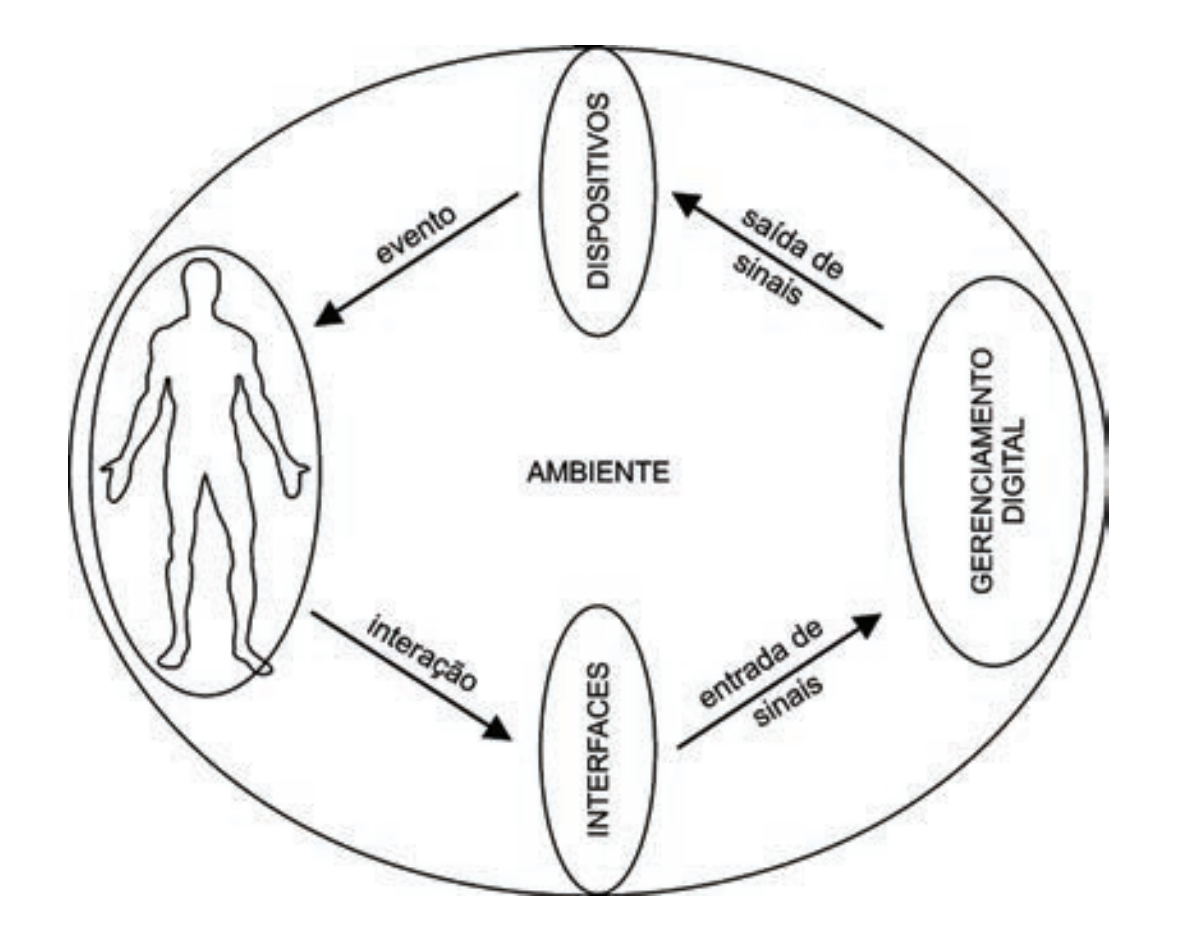
\includegraphics[width=0.8\textwidth]{./04-figuras/instalacoes_interativas}
    \label{fig:instalacoes_interativas}
\end{figure}
\vspace*{-0,9cm}
{\raggedright \fonte{\citeonline{sogabe2011}}}\\


O espaço sempre deve ser considerado para que a obra seja, de fato, uma instalação. De acordo com \citeonline[p. 6]{bochio}, no contexto das instalações interativas, o espaço se torna sensível e os movimentos mais sutis do público são capturados, provocando o diálogo com a imagem. Um evento é tudo que acontece dentro deste espaço. São as respostas fornecidas pelo sistema computacional que se materializam por meio dos dispositivos. Para \citeonline{domingues1998} os dispositivos compõem a cenografia, a
ambientação, mas acima de tudo acrescentam elementos internos à própria concepção
da obra. \citeonline{sogabe2011} afirma que a simples presença do público no espaço, através do andar, ou de alguma ação física, pode gerar alterações no ambiente. Essas alterações são controladas por algum sistema computacional, ou como denomina o autor, através de gerenciamento digital, que recebe as informações, processa e devolve para o ambiente no formato de informações atualizadas, provocando um novo ciclo.


A instalação interativa entende o público como essencial para o acontecimento da obra. O público é um elemento físico presente na instalação e que o artista tem de considerar como parte da instalação \cite[p. 64]{sogabe2011}. Sendo assim, público e interatividade estão intimamente conectados tendo em vista que que a interação se manifesta em alguma ação proposta pelo interator. Sobre a relação do público com o espaço \citeonline[p. 6]{bochio} relata que

\begin{citacao}
Em seus deslocamentos pelo espaço, o público constrói uma trama de relações com a obra por aproximação, afastamento, retornos, paradas, transformando o que é percebido por ele. Em instalações interativas, além disso, o público tem a possibilidade de agir e interagir com a situação proposta promovendo modificações nas próprias imagens e sons:  há transformações de ordem física e não mais apenas perceptiva – o que caracteriza o termo interativo nas instalações.  \cite[p. 6]{bochio}  
\end{citacao}

Para \citeonline[p. 6]{bochio}, as instalações interativas, oferecem além de imagens ou sons, interfaces de acesso ao público, permitindo que à sua ação sejam produzidas respostas em tempo real por parte das máquinas. De acordo com \citeonline{witt}, para que qualquer tipo de interatividade aconteça, é preciso de uma interface, uma tecnologia que propicie a comunicação entre o sistema e o interator. Segundo \citeonline[p. 66]{sogabe2011} "a interface é o aparato físico que capta as ações do público na instalação, a parte sensível do sistema tecnológico". Afirma ainda que a interface não é só um aparato tecnológico, mas está diretamente relacionada à produção da poética da instalação. \citeonline{witt} destacam que estas interfaces devem sempre evoluir, num sentido em que se tornem cada vez mais próximas ao nosso corpo, tenham um funcionamento simples de aprender, e que, acima de tudo, sejam capazes de atender às necessidades da obra.

O gerenciamento digital é realizado geralmente por um micro-controlador digital e um programa, que permitem que as informações enviadas pelos dispositivos sensíveis sejam recebidas, enviadas ao programa que, por sua vez, decide o que fará com essas informações e realiza saídas de informações para os dispositivos. \cite[p. 66]{sogabe2011}

Nota-se que a maneira pela qual a instalação interativa se estrutura é decorrente tanto da poética proposta pelo artista, como pela estrutura tecnológica utilizada, ambas articuladas entre si. \cite[p. 6-7]{bochio}

As instalações interativas com recursos computacionais através de interfaces permitem
a interatividade no sentido stricto do termo. As tecnologias digitais abrem a
possibilidade para o visitante de interagir com o que é proposto promovendo mutações
no próprio tecido luminoso das imagens, modificando sons, andando entre várias
ramificações das imagens, podendo escolher percursos. As tecnologias interativas
promovem mutações de ordem física sobre o mundo virtual eletrônico. Através de
interfaces o corpo entra numa fronteira compartilhada com as máquinas ampliando o
campo de percepção. \cite{domingues1998}


A instalação vem para romper com a hegemonia absoluta da frontalidade da pintura
e o rompimento definitivo com o pedestal na escultura para propor um espaço expandido,
penetrável, participativo e ambíguo deslizando entre as fronteiras da materialidade
e da imaterialidade. \cite[p. 1130]{semeler2015}

Ao invés de absorver o meio passivamente a instalação irá implicar em sua anexação/relação.
Por vezes, a escolha do lugar é inseparável da obra. Noutras, o meio
irá se opor a mesma. No entanto, nunca será indiferente ao espaço agregado ao
tempo ou construção do espaço pelo tempo. \cite[p. 1130]{semeler2015}

O espectador é recrutado por meio da interatividade para que exerça um papel ativo na construção da obra.\cite[p. 1140]{semeler2015}


